\documentclass{../res/univ-projet}

%Import des packages utilisés pour le document
\usepackage[utf8x]{inputenc}
\usepackage[francais]{babel}
\usepackage[T1]{fontenc}
\usepackage{listings}
\usepackage[T1]{fontenc}
\makeatletter
\newcommand\verbfile[1]{%
	\begingroup
		\let\do\@makeother\dospecials
		\parindent\z@\obeyspaces\ttfamily
		\catcode`\^^M\active
		\begingroup\lccode`\~`\^^M \lowercase{\endgroup\def~{\par\leavevmode}}%
		\input#1\relax
	\endgroup
}
\makeatother

%\usepackage{array}
%\usepackage{hyperref}
%\usepackage{tabularx, longtable}
%\usepackage[table]{xcolor}
%\usepackage{fancyhdr}
%\usepackage{lastpage}

\definecolor{gris}{rgb}{0.95, 0.95, 0.95}
\definecolor{listinggray}{gray}{0.4}
\definecolor{lbcolor}{rgb}{0.91,0.91,0.91}
\lstset{
	backgroundcolor=\color{lbcolor},
	tabsize=3,
	rulecolor=,
	%fillcolor=\color{lbcolor},,
        basicstyle=\scriptsize,
        %basicstyle=\ttfamily,
        upquote=true,
        aboveskip={0.8\baselineskip},
        %columns=fixed,
        showstringspaces=false,
        numbers=left ,numberstyle=\tiny\bfseries ,
        stepnumber=1,
        firstnumber=1,
        numberfirstline=true
    	numbersep=16pt,
        extendedchars=true,
        breaklines=true,
        columns=flexible,
        prebreak = \raisebox{0ex}[0ex][0ex]{\ensuremath{\hookleftarrow}},
        frame=single,
        %frameround=ffff,
        %framerule=0.05cm,
        showtabs=false,
        showspaces=false,
        showstringspaces=false,
        identifierstyle=\ttfamily,
        %keywordstyle=\color[rgb]{0,0,1},
        keywordstyle=\bfseries\ttfamily\color[rgb]{0,0,1},
        commentstyle=\color[rgb]{0.133,0.545,0.133},
        %stringstyle=\color[rgb]{0.627,0.126,0.941},
        stringstyle=\ttfamily\color[rgb]{0.627,0.126,0.941},
}

%Redéfinition des marges
%\addtolength{\hoffset}{-2cm}
%\addtolength{\textwidth}{4cm}
\addtolength{\topmargin}{-1cm}
\addtolength{\textheight}{1cm}
\addtolength{\headsep}{0.8cm} 
\addtolength{\footskip}{-0.2cm}


%Import page de garde et structures pour la gestion de projet
%\usepackage{structures}

%Variables
\logo{../res/logo_univ.png}
\title{Spécification Technique de Besoin}
\author{Kheireddine \bsc{Berkane}, Nasser \bsc{Adjibi}}
\projet{Compilateur LLVM}
\projdesc{Langage jouet Kawa}
\filiere{M1GIL - Conduite de Projet}
\version{0.7}
\relecteur{Pierre-Luc \bsc{BLOT}, Alexandre \bsc{PETRE}}
%\signataire{Florent \bsc{NICART}}
\date{\today}

\histentry{0.1}{04/11/2014}{Version initiale.}
\histentry{0.1.5}{18/11/2014}{Définition des cas d'utilisations et des exigences.}
\histentry{0.2}{03/12/2014}{Modifications par rapport au retour client du 25/11/2014.}
\histentry{0.3}{10/12/2014}{ \begin{itemize}
								 \item Les parties événements déclenchants ont été détaillées.
								 \item Les parties flots d'exceptions, ainsi que les conditions d’arrêts de toutes les exigences fonctionnelles ont été détaillées.
								 \item L'ajout des exigences opérationnelles d'interface.
								 \item Correction des erreurs signalées lors de la réunion client 04/12/2014.	
							 \end{itemize}	 	
								 }
\histentry{0.4}{22/12/2014}{ \begin{itemize}
\item Les parties événements déclenchants ont été modifiées et structurées sous forme d'une liste.
\item Les parties flots d'exceptions, ainsi que les conditions d’arrêts de toutes les exigences fonctionnelles ont été été modifiées et structurées sous forme d'une liste.
\item La suppression des exigences opérationnelles d'interface après une remarque faite par le prof du TP gestion de projet.
\item Changement de priorité de l'exigence fonctionnelle EF\_4 en secondaire car elle dépend de l'exigence EF\_3 qui est secondaire.
\item Correction des erreurs signalées lors du retour client par mail le 19/12/2014.	
\end{itemize}	 	
}
\histentry{0.5}{18/01/2015}{ \begin{itemize}
\item Élimination des exigences de réalisations qui correspondent aux exigences fonctionnelles afin d'éviter les redondances inutiles. 
\item La partie des exigences fonctionnelles a été détaillée ainsi que les scénarios des exceptions ont été spécifiés afin de faciliter les tests après.
\item Modifications apportées par rapport à la revue du lancement du projet 19/01/2015.
\end{itemize}
}
\histentry{0.6}{11/04/2015}{ 
\begin{itemize}
\item Élimination de l'exigence fonctionnelle EF\_3 : Compiler une application en mode partagé 
\item Élimination de l'exigence fonctionnelle EF\_4 : Compiler une bibliothèques partagée
\item Élimination de l'exigence fonctionnelle EF\_6 : Indiquer les chemins des dépendances entre le source de l'application et des modules (classe/interface) externes
\item Élimination de l'exigence de réalisation EXR\_4 : Compilation d'application partagée
\item Élimination de l'exigence de réalisation EXR\_6 : Compilation de bibliothèque partagée
\item Élimination de l'exigence de réalisation EXR\_25 : Définition d'attributs ou de variables de type \textbf{value}
\item Élimination de l'exigence de réalisation EXR\_26 : Définition méthode value
\item Élimination de l'exigence de réalisation EXR\_41 :  Gestion des exceptions
\item Changement du diagramme de cas d'utilisation après la discussion avec client afin de réduire quelques exigences fonctionnelles et de réalisation 
\end{itemize}
}

\newpage
\histentry{0.7}{15/04/2015}{ 
\begin{itemize}
\item Mettre l'exigence fonctionnelle EF\_3 : Afficher la version du compilateur en secondaire
\item Élimination de l'exigence fonctionnelle EF\_4 :Activer l'affichage en couleur
\item Élimination de l'exigence de réalisation EXR\_5 : Garbage collector
\end{itemize}
}


% -- Début du document -- %
\begin{document}

%Page de garde
\maketitle
\newpage
%La table des matières
\tableofcontents
\newpage
\section{Analyse lexicale}
\subsection{Objectif de l'analyse lexicale}
le principale objectif de cette analyse est de reconnaitre des unités lexicales (tokens).
Chaque token est défini par une expression rationnelle, les entités reconnues lors de cette phase serviront par la suite comme entrée de la phase d'analyse syntaxique.

\subsection{Lexer}
\verbfile {lexer.txt}



\newpage
\section{Analyse syntaxique}
\subsection{Objectif de l'analyse syntaxique}
% Présentation succinte du sujet et hyp de travail.
l'objectif de l'analyse syntaxique est de reconnaître les phrases appartenant à la syntaxe du langage
son entrée est le flot des lexèmes construits par l'analyse lexicale, sa sortie est un arbre de syntaxe abstraite représentant le programme. Elle permet d'identifier et de localiser les erreurs de syntaxe du langage pour notre cas le langage source est le langage jouet kawa.\\

\subsection{Grammaire du langage kawa}
Afin de spécifier et de générer le langage kawa nous avons défini une grammaire non ambigüe permettant d'engendrer toute la syntaxe du langage source, cette grammaire permettra par la suite de construire l'arbre de syntaxe abstraite qui lui sera utile pour la prochaine phase d'analyse sémantique.\\
Notre grammaire est constituée d'un ensemble de règles de productions :\\

% \input{grammaire.txt} %inclus par \jobname .tex
\verbfile {grammaire.txt}
% Bloc Grammaire


%END Bloc grammaire

\subsection{Construction de l'arbre abstrait} 
 Nous construisons à travers cette phase d'analyse un arbre abstrait de syntaxe qui sera utilisé par les prochaines phases d'analyse (la sémantique et la génération de code intermédiaire). L'analyse sémantique a pour objectif de vérifier le sens de l'arbre monté en mémoire et de le décorer en ajoutant des informations nécessaires pour la génération de code intermédiaire.\\
 
Dans le cadre de ce projet nous avons opté pour une solution qui produit un seul arbre en mémoire \textbf{KawaTree} qui est une collection de classe. Ce même KawaTree sera utilisé par l'ensemble des modules, chacun de ces modules possèdent une interface de connexion avec l'arbre pour extraire les informations nécessaires à cette phase d'analyse.\\

Notre objectif pendant cette phase est de construire et de produire le KawaTree afin de permettre aux autres modules de continuer la chaine de compilation en prenant en paramètre d'entrée le KawaTree qui est un arbre abstrait commun pour tous les modules

Nous présentons le diagramme de classe (KawaTree)ainsi que des classes qui ont une relation avec ce diagramme mais qui ne sont utilisées que par le module syntaxique:

\begin{figure}[h!]
\centering
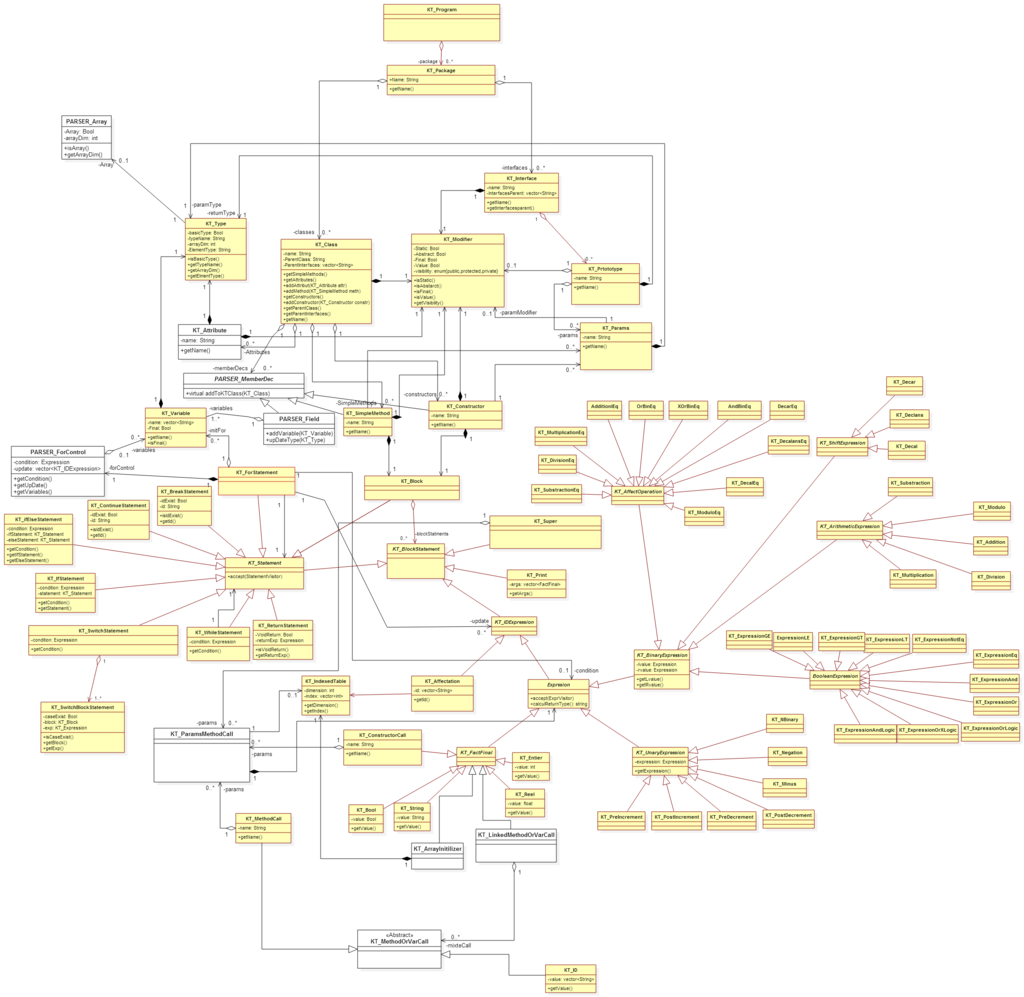
\includegraphics[scale=0.20]{parser_ktdiagramme.png}
\caption[KawaTree avec des classes du parser.]{KawaTree avec des classes du parser.}
\end{figure}
  
  \newpage
 \subsection{Outils de réalisation} 
 Afin de réaliser le module d'analyse syntaxique nous avons utilisé les deux outils:
 \begin{itemize}
 \item  \textbf{Flex}: c'est une version de lex qui est un générateur d'analyse lexical, nous pouvons définir à travers cet outil des unités lexicales pour les reconnaitre après dans un processus de compilation d'un programme source.
\item \textbf{GNU Bison}: est l'implémentation GNU du compilateur de compilateur yacc, spécialisé dans la génération d'analyseurs syntaxiques, il permet de définir la grammaire du langage source ainsi que de produire un analyseur syntaxique en déclenchant les actions des règles de productions invoquées par le programme source, les règles de production sont déclenchés de bas vers le haut car bison est basé sur un analyse ascendante c'est la méthode d'analyse la plus performante.
 
\end{itemize}   ~\\
Nous utiliserons ces deux outils Flex et Bison dans cette phase d'analyse syntaxique car le bison prend en paramètre d'entré les lexèmes qui ont été défini dans Flex afin de produire un arbre abstrait de syntaxe ce dernier sera généré en c++.


\end{document}

